\documentclass{article}

%%
%% \BibTeX command to typeset BibTeX logo in the docs
\AtBeginDocument{%
  \providecommand\BibTeX{{%
    \normalfont B\kern-0.5em{\scshape i\kern-0.25em b}\kern-0.8em\TeX}}}


%%
%% end of the preamble, start of the body of the document source.
\usepackage{textcomp}
\usepackage{multirow}
\usepackage{array}
\usepackage{graphicx}
\usepackage{booktabs}
\usepackage{blindtext}
\usepackage[ngerman]{babel}
\usepackage{hyperref}
\usepackage[table,xcdraw]{xcolor}
\usepackage{colortbl}

\hypersetup{
    colorlinks=true,     % true: colored links, false: red boxes
    linkcolor=black,      % color of internal links
    citecolor=black,     % color of citation links
    urlcolor=black     % color of URL links
}

\newcolumntype{M}[1]{>{\centering\arraybackslash}m{#1}}
%Definition of Colors - Start
\pagestyle{plain}

\begin{document}

\title{Aufgabenstellung 1 Taucher}

\begin{figure}
    \centering
    
\includegraphics[width=0.5\textwidth]{fig/Fig1.png}
    \label{fig:title-image}
\end{figure}


\author{Harald Beier (\lowercase{2410781028@hochschule-burgenland.at})}

\author{\\Susanne Peer (\lowercase{2410781002@hochschule-burgenland.at})}

\author{\\Patrick Prugger (\lowercase{2410781029@hochschule-burgenland.at})}




\maketitle

\newpage
\renewcommand{\contentsname}{Inhaltsverzeichnis}
\tableofcontents
\newpage
\section{Projektumsetzung und Dokumentation}

\subsection{Projektübersicht}

Dieses Dokument beschreibt die High-Level-Umsetzung eines modernen DevOps-Projekts mit Fokus auf automatisierte CI/CD-Pipelines, Qualitätssicherung und kontinuierliche Integration. Das Projekt implementiert eine vollständige Notes-API-Anwendung mit umfassender Testabdeckung und automatisierter Deployment-Pipeline.

\subsubsection{Technologie-Stack}
\begin{itemize}
    \item \textbf{Backend}: Node.js mit Express.js Framework
    \item \textbf{Testing}: Jest für Unit- und Integrationstests
    \item \textbf{CI/CD}: GitHub Actions
    \item \textbf{Code Quality}: SonarQube für statische Code-Analyse
    \item \textbf{Dependency Management}: Dependabot für automatisierte Updates
    \item \textbf{Containerization}: Docker mit Multi-Stage Builds
    \item \textbf{Registry}: GitHub Container Registry (GHCR)
\end{itemize}

\subsubsection{Repository-Zugang}
Das Projekt ist in einem öffentlichen GitHub Repository verfügbar:
\begin{itemize}
    \item \textbf{Repository URL}: \url{https://github.com/Gruppe1DevOps/DevOpsG1}
    \item \textbf{Hauptbranch}: main
    \item \textbf{Anwendungscode}: \texttt{Taucher/PT/Code/}
    \item \textbf{CI/CD Konfiguration}: \texttt{.github/workflows/}
\end{itemize}

\subsection{Anwendungsarchitektur}

\subsubsection{Notes API Implementierung}
Die Kern-Anwendung ist eine RESTful API für die Verwaltung von Notizen mit folgenden Endpunkten:

\begin{table}[h!]
    \centering
    \caption{API Endpunkte der Notes-Anwendung}
    \label{tab:api-endpoints}
    \begin{tabular}{|l|l|l|}
    \hline
    \textbf{HTTP Method} & \textbf{Endpoint} & \textbf{Beschreibung} \\ \hline
    GET & /api/notes & Alle Notizen abrufen \\ \hline
    GET & /api/notes/:id & Spezifische Notiz abrufen \\ \hline
    POST & /api/notes & Neue Notiz erstellen \\ \hline
    DELETE & /api/notes/:id & Notiz löschen \\ \hline
    \end{tabular}
\end{table}

\subsubsection{Datenmodell}
Jede Notiz enthält folgende Attribute:
\begin{itemize}
    \item \textbf{id}: Eindeutige Identifikationsnummer (automatisch generiert)
    \item \textbf{content}: Textinhalt der Notiz (erforderlich)
    \item \textbf{important}: Boolean-Wert für Wichtigkeit (optional, Standard: false)
    \item \textbf{date}: Erstellungsdatum (automatisch generiert)
\end{itemize}

\subsection{CI/CD Pipeline Architektur}

\subsubsection{Pipeline-Übersicht}
Die CI/CD-Pipeline implementiert einen mehrstufigen Ansatz mit klarer Trennung der Verantwortlichkeiten:

\begin{figure}[h!]
    \centering
    \caption{CI/CD Pipeline Workflow}
    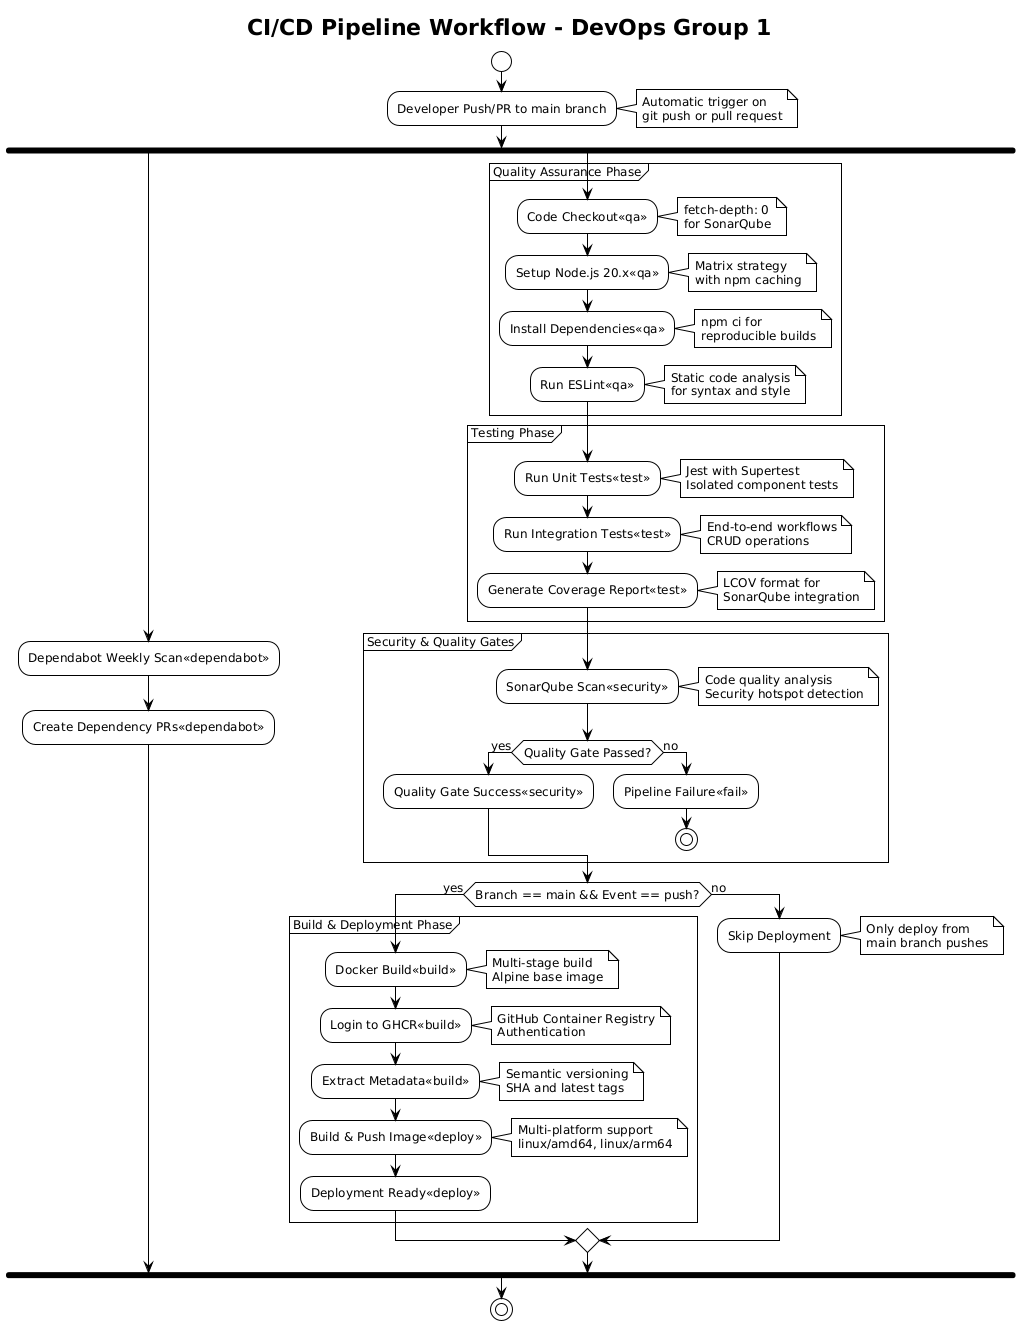
\includegraphics[width=1\textwidth]{fig/cicd-pipeline.png}
    \label{fig:cicd-pipeline}
\end{figure}

\subsubsection{Pipeline-Stufen}

\paragraph{1. Trigger-Phase}
\begin{itemize}
    \item Automatische Auslösung bei Push/Pull Request auf main Branch
    \item Parallele Ausführung für Pull Requests zur Qualitätssicherung
    \item Conditional Deployment nur bei main Branch
\end{itemize}

\paragraph{2. Quality Assurance Phase}
\begin{itemize}
    \item \textbf{Code Checkout}: Vollständiger Git-Verlauf für SonarQube
    \item \textbf{Node.js Setup}: Matrix-Strategie für Version 20.x
    \item \textbf{Dependency Installation}: npm ci für reproduzierbare Builds
    \item \textbf{ESLint}: Statische Code-Analyse für Syntax und Style
\end{itemize}

\paragraph{3. Testing Phase}
\begin{itemize}
    \item \textbf{Unit Tests}: Isolierte Komponententests
    \item \textbf{Integration Tests}: End-to-End Workflow-Tests
    \item \textbf{Coverage Analysis}: Vollständige Test-Coverage-Berichte
\end{itemize}

\paragraph{4. Security und Quality Gates}
\begin{itemize}
    \item \textbf{SonarQube Scan}: Umfassende Code-Qualitätsanalyse
    \item \textbf{Quality Gate}: Automatische Pipeline-Unterbrechung bei Qualitätsproblemen
    \item \textbf{Coverage Threshold}: Mindestens 80\% Test-Coverage erforderlich
\end{itemize}

\paragraph{5. Build und Deployment Phase}
\begin{itemize}
    \item \textbf{Docker Build}: Multi-Stage Containerisierung
    \item \textbf{Registry Push}: Automatischer Upload zu GitHub Container Registry
    \item \textbf{Semantic Versioning}: Automatische Tag-Generierung
\end{itemize}

\subsection{Testing-Strategie}

\subsubsection{Multi-Layer Testing Approach}
Das Projekt implementiert eine umfassende Testing-Strategie mit verschiedenen Test-Ebenen:

\paragraph{Unit Tests}
\begin{itemize}
    \item \textbf{Zweck}: Isolierte Komponententests für einzelne Funktionen
    \item \textbf{Framework}: Jest mit Supertest für HTTP-Testing
    \item \textbf{Coverage}: Fokus auf hohe Code-Coverage einzelner Module
    \item \textbf{Ausführungszeit}: Schnelle Ausführung für sofortiges Feedback
\end{itemize}

\begin{table}[h!]
    \centering
    \caption{Unit Test Abdeckung}
    \label{tab:unit-tests}
    \begin{tabular}{|l|l|}
    \hline
    \textbf{Test Case} & \textbf{Beschreibung} \\ \hline
    GET /api/notes & Abruf aller Notizen mit korrekter Struktur \\ \hline
    POST /api/notes & Erstellung neuer Notizen mit gültigen Daten \\ \hline
    POST /api/notes (invalid) & Fehlerbehandlung bei ungültigen Daten \\ \hline
    GET /api/notes/:id & Abruf spezifischer Notizen \\ \hline
    GET /api/notes/:id (404) & 404-Response für nicht existierende Notizen \\ \hline
    \end{tabular}
\end{table}

\paragraph{Integration Tests}
\begin{itemize}
    \item \textbf{Zweck}: End-to-End Workflow-Tests für komplette User Journeys
    \item \textbf{Scope}: Vollständige CRUD-Operationen und Concurrent Request Handling
    \item \textbf{Datenintegrität}: Verifikation der Datenkonsistenz über mehrere Operationen
    \item \textbf{Performance}: Concurrent Request Testing für Skalierbarkeit
\end{itemize}

\begin{table}[h!]
    \centering
    \caption{Integration Test Szenarien}
    \label{tab:integration-tests}
    \begin{tabular}{|l|l|}
    \hline
    \textbf{Test Szenario} & \textbf{Beschreibung} \\ \hline
    Complete CRUD Workflow & Vollständiger Lebenszyklus einer Notiz \\ \hline
    Concurrent Requests & 5 simultane Notiz-Erstellungen \\ \hline
    Data Consistency & Verifikation der Datenintegrität \\ \hline
    Unique ID Generation & Eindeutige ID-Generierung unter Last \\ \hline
    \end{tabular}
\end{table}

\subsection{Code Quality Management}

\subsubsection{SonarQube Integration}
SonarQube wird für kontinuierliche Code-Qualitätsanalyse eingesetzt:

\paragraph{Konfiguration}
\begin{itemize}
    \item \textbf{Projekt}: DevOps Group 1 - Note App
    \item \textbf{Organisation}: gruppe1devops
    \item \textbf{Platform}: SonarCloud
    \item \textbf{Quality Gate}: Automatische Pipeline-Unterbrechung bei Fehlern
\end{itemize}


\paragraph{Qualitätsmetriken}
Die folgenden Metriken werden von SonarQube überwacht und analysiert:

\begin{table}[h!]
    \centering
    \caption{SonarQube Qualitätsmetriken}
    \label{tab:sonar-metrics}
    \begin{tabular}{|l|l|l|}
    \hline
    \textbf{Metrik} & \textbf{Threshold} & \textbf{Beschreibung} \\ \hline
    Code Coverage & $>$ 80\% & Mindest-Testabdeckung \\ \hline
    Code Smells & 0 & Wartbarkeits-Issues \\ \hline
    Security Hotspots & 0 & Potenzielle Sicherheitslücken \\ \hline
    Duplicated Code & $<$ 3\% & Code-Duplikation \\ \hline
    Cyclomatic Complexity & $<$ 10 & Komplexitätsanalyse \\ \hline
    \end{tabular}
\end{table}

\subsubsection{ESLint Konfiguration}
Statische Code-Analyse für JavaScript/Node.js:
\begin{itemize}
    \item \textbf{Standard}: ESLint 8.x mit modernen JavaScript-Standards
    \item \textbf{Rules}: Konsistente Code-Formatierung und Best Practices
    \item \textbf{Integration}: Automatische Ausführung in CI/CD Pipeline
    \item \textbf{Fail-Fast}: Pipeline-Unterbrechung bei Linting-Fehlern
\end{itemize}

\subsection{Dependency Management}

\subsubsection{Dependabot Konfiguration}
Automatisierte Dependency-Updates für Sicherheit und Aktualität:

\paragraph{NPM Dependencies}
\begin{itemize}
    \item \textbf{Schedule}: Wöchentliche Updates jeden Montag um 09:00
    \item \textbf{PR Limit}: Maximal 10 gleichzeitige Pull Requests
    \item \textbf{Reviewer}: Automatische Zuweisung an t-stefan
    \item \textbf{Commit Format}: Conventional Commits mit "chore" Prefix
\end{itemize}

\paragraph{GitHub Actions Dependencies}
\begin{itemize}
    \item \textbf{Schedule}: Wöchentliche Updates für Action-Versionen
    \item \textbf{PR Limit}: Maximal 5 gleichzeitige Pull Requests
    \item \textbf{Scope}: Alle GitHub Actions im Repository
\end{itemize}

\subsubsection{Security Benefits}
\begin{itemize}
    \item \textbf{Vulnerability Patching}: Automatische Sicherheitsupdates
    \item \textbf{Compliance Tracking}: Aktuelle Dependency-Inventarisierung
    \item \textbf{Risk Mitigation}: Reduzierung bekannter Sicherheitslücken
    \item \textbf{Automated Testing}: Jedes Update wird durch CI/CD validiert
\end{itemize}

\subsection{Containerization und Deployment}

\subsubsection{Docker Implementation}
Multi-Stage Docker Build für optimierte Container:

\paragraph{Build Strategy}
\begin{itemize}
    \item \textbf{Base Image}: node:20-alpine für minimale Größe
    \item \textbf{Multi-Stage}: Separate Build- und Runtime-Stages
    \item \textbf{Security}: Non-root User für Container-Ausführung
    \item \textbf{Optimization}: Layer-Caching für schnellere Builds
\end{itemize}

\paragraph{Container Registry}
\begin{itemize}
    \item \textbf{Registry}: GitHub Container Registry (ghcr.io)
    \item \textbf{Tagging Strategy}: Semantic Versioning mit SHA und Latest Tags
    \item \textbf{Multi-Platform}: Support für linux/amd64 und linux/arm64
    \item \textbf{Caching}: GitHub Actions Cache für Build-Optimierung
\end{itemize}

\subsubsection{Deployment Pipeline}
\begin{table}[h!]
    \centering
    \caption{Deployment Tag-Strategie}
    \label{tab:deployment-tags}
    \begin{tabular}{|l|l|}
    \hline
    \textbf{Tag Type} & \textbf{Format} \\ \hline
    Branch Reference & main \\ \hline
    SHA Reference & main-\{sha\} \\ \hline
    Latest & latest (nur main branch) \\ \hline
    Version & v1.0.\{run\_number\} \\ \hline
    \end{tabular}
\end{table}

\subsection{Monitoring und Wartung}

\subsubsection{Pipeline Health Monitoring}
Kontinuierliche Überwachung der Pipeline-Gesundheit:

\paragraph{Key Performance Indicators}
\begin{itemize}
    \item \textbf{Build Success Rate}: Ziel > 95\%
    \item \textbf{Average Build Time}: Monitoring für Performance-Regression
    \item \textbf{Test Coverage}: Aufrechterhaltung > 80\% Line Coverage
    \item \textbf{Security Vulnerabilities}: Null High-Severity Issues
    \item \textbf{Dependency Freshness}: < 30 Tage hinter aktueller Version
\end{itemize}

\subsubsection{Wartungsplan}
\paragraph{Wöchentliche Aufgaben}
\begin{itemize}
    \item Review von Dependabot Pull Requests
    \item Überprüfung der SonarQube Quality Trends
    \item Monitoring der Build-Performance-Metriken
    \item Review der Security Scan Ergebnisse
\end{itemize}

\paragraph{Monatliche Aufgaben}
\begin{itemize}
    \item Update der GitHub Actions Versionen
    \item Review und Update der Quality Gates
    \item Audit der Secret-Nutzung und Rotation
    \item Performance-Optimierung Review
\end{itemize}

\subsection{Best Practices und Lessons Learned}

\subsubsection{Implementierte Best Practices}
\begin{itemize}
    \item \textbf{Fail-Fast Strategy}: Optimierte Job-Reihenfolge für schnelles Feedback
    \item \textbf{Security-First}: Secrets Management und Least-Privilege Access
    \item \textbf{Caching Strategy}: Dependency und Build-Caching für Performance
    \item \textbf{Parallel Execution}: Matrix-Builds für Effizienz
    \item \textbf{Quality Gates}: Automatische Pipeline-Unterbrechung bei Qualitätsproblemen
\end{itemize}

\subsubsection{Herausforderungen und Lösungen}
\paragraph{SonarQube Integration}
\begin{itemize}
    \item \textbf{Problem}: Quality Gate Timeouts bei großen Projekten
    \item \textbf{Lösung}: Timeout-Konfiguration und selective Scanning
\end{itemize}

\paragraph{Docker Build Optimization}
\begin{itemize}
    \item \textbf{Problem}: Lange Build-Zeiten
    \item \textbf{Lösung}: Multi-Stage Builds und Layer-Caching
\end{itemize}

\paragraph{Test Environment Consistency}
\begin{itemize}
    \item \textbf{Problem}: Unterschiedliche Verhalten zwischen lokaler und CI-Umgebung
    \item \textbf{Lösung}: Containerisierte Test-Umgebungen und Matrix-Builds
\end{itemize}

\subsection{Fazit und Ausblick}

\subsubsection{Projektergebnisse}
Das implementierte DevOps-Projekt demonstriert erfolgreich:
\begin{itemize}
    \item \textbf{Vollautomatisierte CI/CD Pipeline} mit Quality Gates
    \item \textbf{Umfassende Test-Strategie} mit hoher Coverage
    \item \textbf{Kontinuierliche Code-Qualitätssicherung} durch SonarQube
    \item \textbf{Automatisierte Dependency-Verwaltung} für Sicherheit
    \item \textbf{Containerisierte Deployment-Strategie} für Skalierbarkeit
\end{itemize}
\newpage
\renewcommand{\refname}{Literaturverzeichnis}
\addcontentsline{toc}{section}{Literaturverzeichnis}
%% The next two lines define the bibliography style to be used, and
%% the bibliography file.
\bibliographystyle{apalike}
\bibliography{section/references}

\end{document}
\endinput
%%
%% End of file `sample-acmlarge.tex'.
